\documentclass[aspectratio=169,10pt]{beamer}

\usepackage[T1,T2A]{fontenc}
\usepackage[utf8]{inputenc}
\usepackage[english,russian]{babel}
\usepackage{graphicx}
\usepackage{array}
\usepackage{booktabs}

\usetheme{default}
\setbeamertemplate{navigation symbols}{}
\setbeamertemplate{footline}[frame number]
\setbeamercolor{title}{fg=black}
\setbeamercolor{frametitle}{fg=black,bg=white}
\setbeamercolor{normal text}{fg=black,bg=white}
\setbeamercolor{itemize item}{fg=black}
\setbeamerfont{title}{series=\mdseries,size=\Large}
\setbeamerfont{frametitle}{series=\mdseries,size=\large}
\setbeamerfont{footline}{size=\scriptsize}

\newcommand{\smallnote}[1]{\vspace{0.3cm}{\small #1}}
\newcommand{\pipelinebox}[1]{\fbox{\parbox[c][0.62cm][c]{0.68\textwidth}{\centering\small #1}}}

\title{Анализ тональности региональной новостной повестки в контексте целей устойчивого развития}
\author{Тарана Евгения Вячеславович}
\institute{СГУ имени Н. Г. Чернышевского}
\date{2026}

\begin{document}

\begin{frame}
\titlepage
\end{frame}

\begin{frame}{Цель работы}
Цель работы --- разработать и апробировать подход к анализу региональной новостной повестки в контексте целей устойчивого развития.

\smallnote{В работе объединяются три слоя анализа: тематическая классификация по 17 ЦУР, словарная оценка тональности и сопоставление с региональными показателями Росстата.}
\end{frame}

\begin{frame}{Задачи}
\begin{itemize}
\item классифицировать региональные VK-сообщения по 17 целям устойчивого развития;
\item агрегировать цели в социальную, экономическую и экологическую категории;
\item оценить тональность текстов с помощью словаря КартаСловСент;
\item сравнить регионы по структуре и тональности SDG-повестки;
\item сопоставить характеристики повестки с показателями Росстата.
\end{itemize}
\end{frame}

\begin{frame}{Этапы обработки}
\centering
\setlength{\fboxsep}{4pt}
\pipelinebox{Региональные сообщения VK}\\[-0.02cm]
$\downarrow$\\[-0.02cm]
\pipelinebox{SDG-классификация RuBERT}\\[-0.02cm]
$\downarrow$\\[-0.02cm]
\pipelinebox{Группировка 17 ЦУР в 3 категории}\\[-0.02cm]
$\downarrow$\\[-0.02cm]
\pipelinebox{Словарная оценка тональности}\\[-0.02cm]
$\downarrow$\\[-0.02cm]
\pipelinebox{Агрегация по регионам и годам}\\[-0.02cm]
$\downarrow$\\[-0.02cm]
\pipelinebox{Росстат, Кендалл, FE-регрессия}
\end{frame}

\begin{frame}{RuBERT-классификация}
\begin{itemize}
\item базовая модель: DeepPavlov/rubert-base-cased;
\item выходной слой: 17 классов, по одному на каждую ЦУР;
\item тренировочная выборка: OSDG Community Dataset и SDGi Corpus, около 27 тыс. текстов после предобработки;
\item обучение: 6 эпох, Adam, learning rate $2 \cdot 10^{-5}$;
\item качество на тестовой выборке: F1 = 0.884;
\item VK-выборка использовалась для проверки применимости модели к региональным новостям.
\end{itemize}
\end{frame}

\begin{frame}{Распределение по 17 ЦУР}
\centering
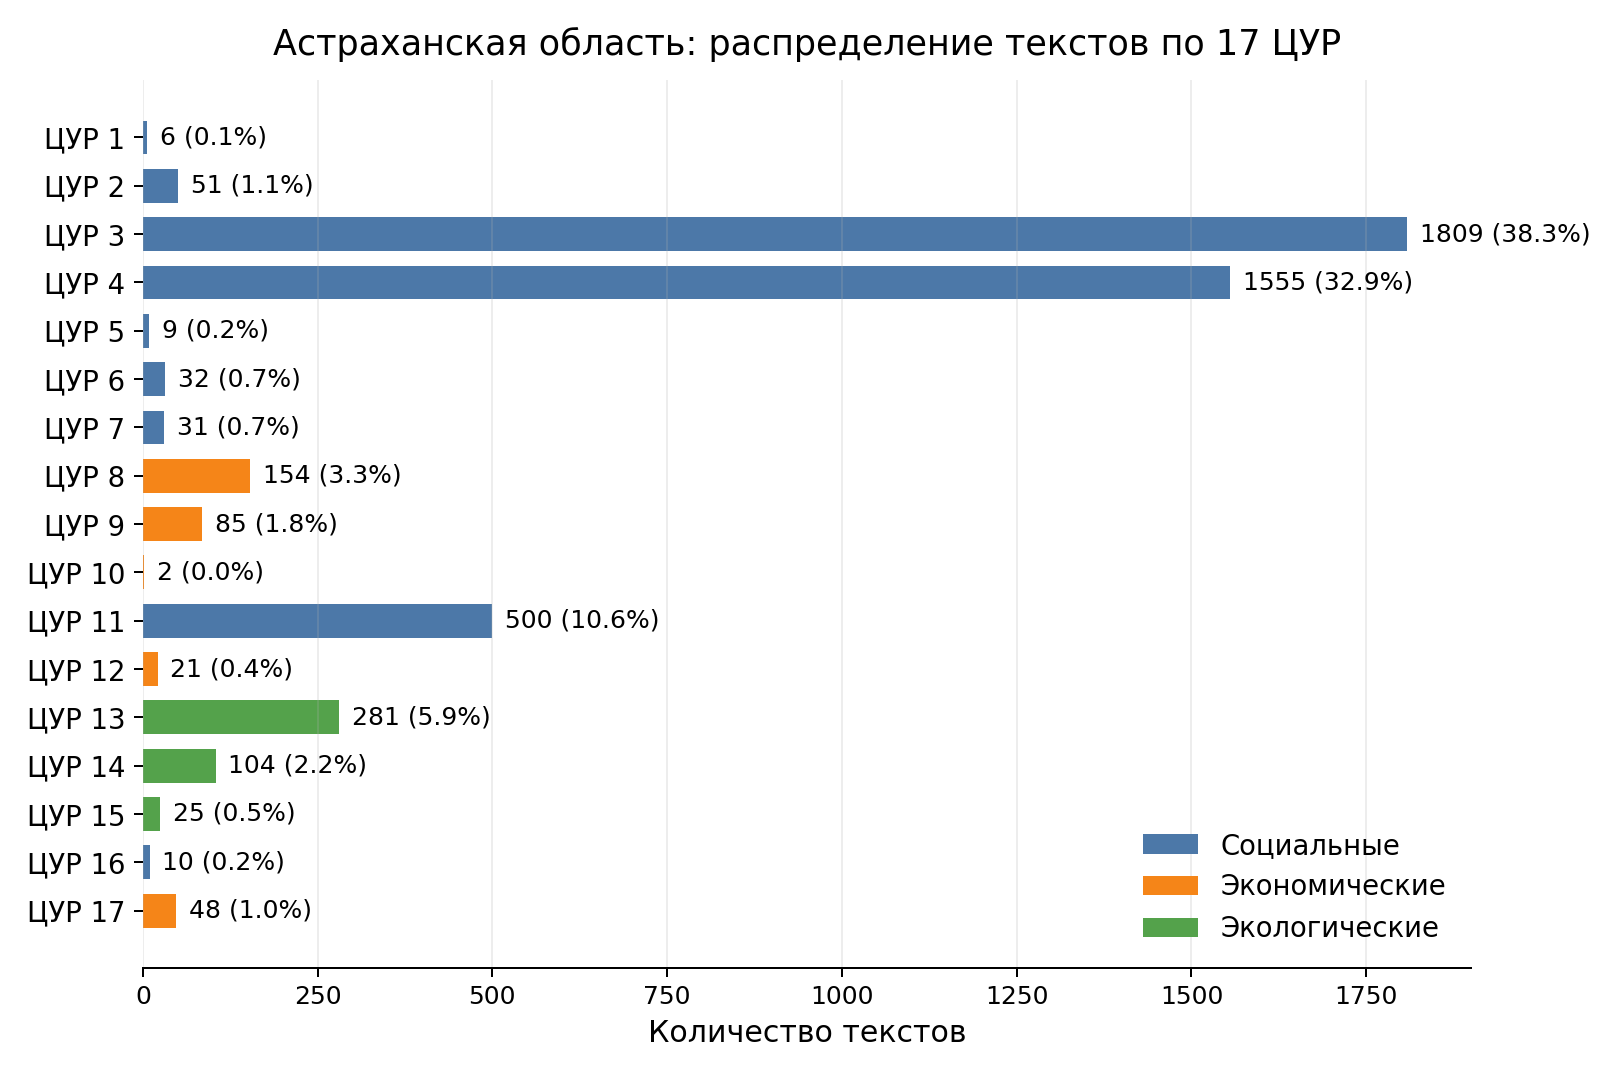
\includegraphics[width=0.70\textwidth]{fig_sdg17_astrakhan.png}

\vspace{0.05cm}
\small Астраханская область, 2020--2025, 4 723 текста.
\end{frame}

\begin{frame}{Группировка ЦУР}
\begin{columns}[T,onlytextwidth]
\begin{column}{0.32\textwidth}
\centering
Социальные

\vspace{0.2cm}
\small ЦУР 1, 2, 3, 4, 5, 6, 7, 11, 16
\end{column}
\begin{column}{0.32\textwidth}
\centering
Экономические

\vspace{0.2cm}
\small ЦУР 8, 9, 10, 12, 17
\end{column}
\begin{column}{0.32\textwidth}
\centering
Экологические

\vspace{0.2cm}
\small ЦУР 13, 14, 15
\end{column}
\end{columns}

\smallnote{Такая группировка позволяет перейти от 17 отдельных классов к сопоставимым макрокатегориям региональной повестки.}
\end{frame}

\begin{frame}{Таблица 5. Показатели Росстата}
\centering
\tiny
\renewcommand{\arraystretch}{1.12}
\resizebox{\textwidth}{!}{%
\begin{tabular}{lrrrrr}
\toprule
Регион и год & ВРП на душу & Безраб., \% & Инвестиции & Зарплата & Выбросы \\
\midrule
Астраханская обл., 2020 & 541 099 & 7.9 & 115 116 & 38 885 & 112 \\
Астраханская обл., 2021 & 688 988 & 7.8 & 115 484 & 42 096 & 91 \\
Астраханская обл., 2022 & 800 576 & 7.1 & 87 352 & 47 780 & 104 \\
Астраханская обл., 2023 & 819 952 & 4.4 & 89 373 & 53 964 & 100 \\
Омская обл., 2020 & 407 371 & 8.9 & 200 450 & 37 828 & 147 \\
Омская обл., 2021 & 426 872 & 6.5 & 191 473 & 41 152 & 159 \\
Омская обл., 2022 & 503 176 & 5.3 & 194 431 & 46 952 & 165 \\
Омская обл., 2023 & 578 934 & 3.6 & 208 399 & 55 227 & 159 \\
Татарстан, 2020 & 658 312 & 3.6 & 615 593 & 39 761 & 325 \\
Татарстан, 2021 & 883 564 & 2.7 & 689 232 & 45 800 & 323 \\
Татарстан, 2022 & 1 035 953 & 2.3 & 888 649 & 52 274 & 320 \\
Татарстан, 2023 & 1 145 174 & 2.1 & 1 180 448 & 61 894 & 320 \\
\bottomrule
\end{tabular}}
\end{frame}

\begin{frame}{Таблица 6. Характеристики повестки}
\centering
\tiny
\renewcommand{\arraystretch}{1.12}
\resizebox{\textwidth}{!}{%
\begin{tabular}{lrrrrrr}
\toprule
Регион и год & Соц., \% & Экон., \% & Экол., \% & +Соц., \% & +Экон., \% & +Экол., \% \\
\midrule
Астраханская обл., 2020 & 91.6 & 2.6 & 5.7 & 54.5 & 92.0 & 75.9 \\
Астраханская обл., 2021 & 88.5 & 3.8 & 7.7 & 77.7 & 92.6 & 76.4 \\
Астраханская обл., 2022 & 86.7 & 6.8 & 6.5 & 83.8 & 93.8 & 82.3 \\
Астраханская обл., 2023 & 82.3 & 5.1 & 12.6 & 83.8 & 97.8 & 64.9 \\
Омская обл., 2020 & 75.9 & 17.6 & 6.5 & 83.7 & 86.0 & 38.1 \\
Омская обл., 2021 & 80.3 & 15.1 & 4.6 & 84.8 & 88.9 & 18.2 \\
Омская обл., 2022 & 72.0 & 20.0 & 8.0 & 88.1 & 95.7 & 92.9 \\
Омская обл., 2023 & 77.5 & 18.5 & 4.0 & 92.5 & 96.7 & 100.0 \\
Татарстан, 2020 & 81.3 & 15.3 & 3.4 & 83.6 & 92.5 & 100.0 \\
Татарстан, 2021 & 64.6 & 13.6 & 21.7 & 61.0 & 85.1 & 29.7 \\
Татарстан, 2022 & 65.0 & 16.8 & 18.2 & 65.1 & 81.0 & 33.3 \\
Татарстан, 2023 & 66.7 & 18.4 & 14.9 & 70.3 & 87.4 & 40.8 \\
\bottomrule
\end{tabular}}
\end{frame}

\begin{frame}[shrink=4]{Таблица 7. Корреляции Кендалла}
\centering
\tiny
\renewcommand{\arraystretch}{0.96}
\resizebox{\textwidth}{!}{%
\begin{tabular}{llrr}
\toprule
Характеристика повестки & Показатель Росстата & $\tau$ & $p$ \\
\midrule
Доля соц. кат., \% & Врачи на 10 тыс. & 0.76 & 0.001 \\
Доля экон. кат., \% & Рождаемость & -0.72 & 0.001 \\
Доля соц. кат., \% & Койки на 10 тыс. & 0.70 & 0.002 \\
Доля соц. кат., \% & Сброс сточных вод & -0.68 & 0.002 \\
Доля соц. кат., \% & Расходы на охрану среды & -0.64 & 0.003 \\
Доля экон. кат., \% & Расходы на охрану среды & 0.64 & 0.003 \\
Доля соц. кат., \% & Выбросы в атмосферу & -0.59 & 0.009 \\
Доля соц. кат., \% & Инвестиции на душу & -0.58 & 0.009 \\
Доля соц. кат., \% & Розница на душу & -0.55 & 0.014 \\
Доля соц. кат., \% & Безработица & 0.53 & 0.016 \\
Позитивность соц., \% & Рождаемость & -0.52 & 0.019 \\
Доля экон. кат., \% & Уловленные загрязнители & 0.50 & 0.023 \\
Позитивность экон., \% & Инвестиции на душу & -0.46 & 0.045 \\
Позитивность экон., \% & Врачи на 10 тыс. & 0.45 & 0.045 \\
Доля экол. кат., \% & ВРП на душу & 0.44 & 0.046 \\
\bottomrule
\end{tabular}}

\vspace{0.05cm}
\scriptsize Показаны пары с $|\tau| > 0.40$, $n=12$.
\end{frame}

\begin{frame}{Основные тезисы}
\begin{itemize}
\item во всех регионах доминирует социальная повестка;
\item экономическая категория имеет наиболее высокую долю позитивных текстов;
\item экологическая категория менее позитивна и сильнее зависит от локальных инфоповодов;
\item структура повестки заметнее связана с показателями Росстата, чем тональность;
\item результаты следует трактовать как предварительные ассоциации, а не как причинные выводы.
\end{itemize}
\end{frame}

\end{document}
